% This file was created by matplotlib2tikz v0.7.4.
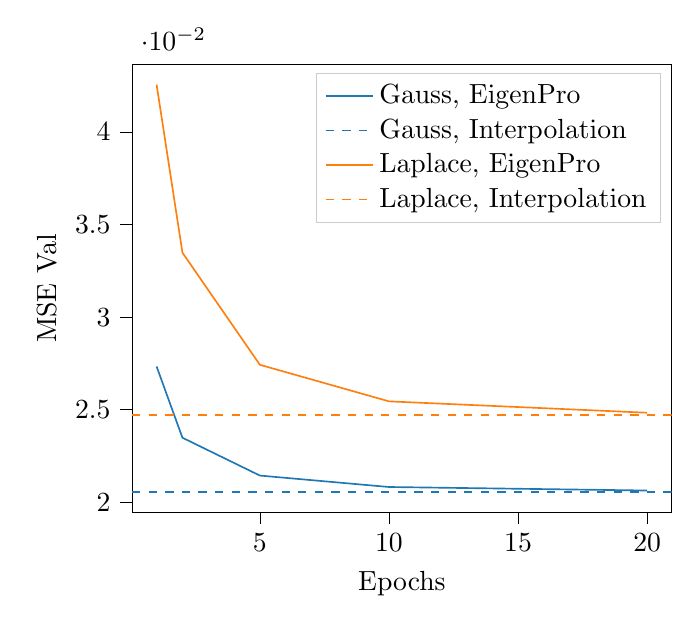
\begin{tikzpicture}

\definecolor{color0}{rgb}{0.12156862745098,0.466666666666667,0.705882352941177}
\definecolor{color1}{rgb}{1,0.498039215686275,0.0549019607843137}

\begin{axis}[
legend cell align={left},
legend style={draw=white!80.0!black},
tick align=outside,
tick pos=left,
x grid style={white!69.01960784313725!black},
xlabel={Epochs},
xmin=0.0499999999999999, xmax=20.95,
xtick style={color=black},
y grid style={white!69.01960784313725!black},
ylabel={MSE Val},
ymin=0.0194391579117425, ymax=0.0436663958534076,
ytick style={color=black}
]
\addplot [semithick, color0]
table {%
1 0.0273320502251387
2 0.0234821424603462
5 0.0214356774359941
10 0.0208179115436971
20 0.0206277057625353
};
\addlegendentry{Gauss, EigenPro}
\addplot [semithick, color0, dashed]
table {%
0.0499999999999998 0.020540396
20.95 0.020540396
};
\addlegendentry{Gauss, Interpolation}
\addplot [semithick, color1]
table {%
1 0.0425651577651501
2 0.0334836662262678
5 0.0274220125839114
10 0.0254457658916712
20 0.0248312373891473
};
\addlegendentry{Laplace, EigenPro}
\addplot [semithick, color1, dashed]
table {%
0.0499999999999998 0.024726693
20.95 0.024726693
};
\addlegendentry{Laplace, Interpolation}
\end{axis}

\end{tikzpicture}